% !TeX spellcheck = en_US
\documentclass[letterpaper,12pt,twoside]{report}
\usepackage{fancyhdr}
\usepackage{fullpage}
\usepackage{tikz}
\usepackage{amsmath}

\begin{document}
	\pagestyle{fancy}
	\fancyhf{}
	\fancyhead[L]{Day 14}
	\fancyhead[R]{\textit{The Calendar Project}}
	\fancyfoot[L]{Citations Involved: none}
	
	% Problem
	\paragraph{Problem}
	\begin{quote}
		\textsf{Mathematician Charles L. Dodgson (Lewis Carroll) died on the 14th in 1891. His book \textit{A Tangled Tale} opens with the following ``know'': ``Two travelers spend
			from 3 o'clock [p.m.] till 9 [p.m.] in
			walking along a level road, up a hill, and
			home again: their pace on the level being
			4 miles an hour, up hill 3, and down hill 6.
			Find distance walked.''}
	\end{quote}
	
	% Graphics
	\begin{center}
		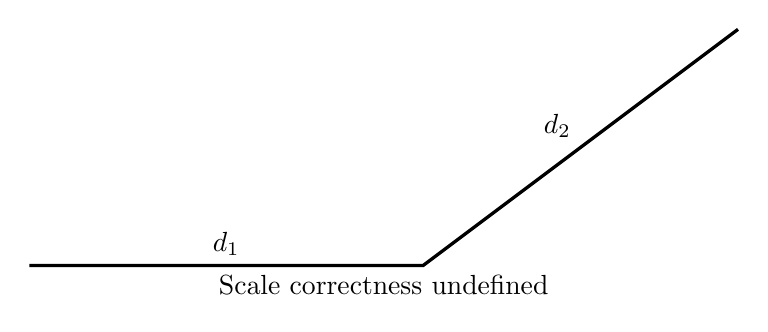
\begin{tikzpicture}
		
		\draw[very thick] (0,0) -- (5,0) -- (9,3);
		\node[above] at (2.5,0) {$d_1$};
		\node[above left] at (7,1.5) {$d_2$};
		\node[below] at (4.5,0) {Scale correctness undefined};
		
		\end{tikzpicture}
	\end{center}
	
	% Reasoning
	\paragraph{Reasoning}
	\begin{quotation}
		
		Let $d_1$ be the length of the level road, and let $d_2$ be the length of the hill. $t=\frac{d}{v}$ where $d$ is the distance traveled, $v$ is the speed of travel, and $t$ is the time spent traveling (derived from $d=vt$). Using this equation with the provided data, the total time spent traveling can be expressed as $\frac{d_1}{4}+\frac{d_2}{3}+\frac{d_2}{6}+\frac{d_1}{4}=6$. It is simplified and transformed as follows:
		
		\begin{center}
			\begin{tabular}{l | l}
				$\frac{d_1}{4}+\frac{d_1}{4}+\frac{d_2}{3}+\frac{d_2}{6}=6$ & Gather like terms \\
				$\frac{2d_1}{4}+\frac{2d_2}{6}+\frac{d_2}{6}=6$ & Add \& match denominators for addition \\
				$\frac{d_1}{2}+\frac{3d_2}{6}=6$ & Simplify \& add \\
				$\frac{d_1}{2}+\frac{d_2}{2}=6$ & Simplify \\
				$d_1+d_2=12$ & Multiply both sides by 2
			\end{tabular}
		\end{center}
	
	Since the travelers walked across both segments twice (in each direction), their total distance traveled is $d_1+d_2+d_2+d_1=12+12=\boxed{24 \text{mi}}$.
	\end{quotation}
	
\end{document}